% ===== 原文 pp.105–117（PDF p.120–132）=====
% 第 3 章 §3.2 末（pp.105–111）、§3.3（pp.112–116）、§3.4 开头（p.117）
% tag 区间：3.4–3.5（式 (3.4) 在 p.111，式 (3.5) 在 p.112）
% 本块不含章标题；§3.3 标题在 p.112 首次出现，由本块写出。

% [原文 p.105]
这仍然是因为 $\mathbb{A}^1_k$ 上在 $0$ 之外可逆的函数拉回到 $X$ 上，是在 $D$ 之外可逆的函数。把这些对数结构分别限制到 $D$ 与 $0$ 上，便得到一个对数态射
\[
  \pi_0: D^{\dagger}\longrightarrow \operatorname{Spec} k^{\dagger}.
\]
按例 3.16 的说法，这个对数态射由 $\mathcal{M}_D$ 的一个截面决定，该截面是把 $\mathcal{M}_{(X,D)}$ 的截面 $z^{(1,1)}$ 限制到 $D$ 上所得。

对整数 $d>0$，令 $\eta_d:\operatorname{Spec} k^{\dagger}\to\operatorname{Spec} k^{\dagger}$ 为满足
\[
  \eta_d^{\#}(c,\beta)=(c,d\beta)
\]
的对数态射。它可以看成 $d$ 次基变换，因为它由对数概形的态射
\[
  \xi_d:(\mathbb{A}^1_k)^{\dagger}\longrightarrow(\mathbb{A}^1_k)^{\dagger}
\]
诱导，而在概形层面上该态射由环同态 $x\mapsto x^d$ 给出。

现在考虑对数点 $f:\operatorname{Spec} k^{\dagger}\to D^{\dagger}$，它给出交换图表
\begin{center}
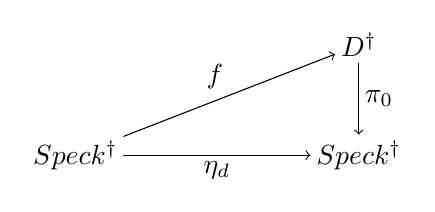
\begin{tikzpicture}[every node/.style={inner sep=2pt}]
  \node (A) at (0,0) {$\operatorname{Spec} k^{\dagger}$};
  \node (B) at (3.6,0) {$\operatorname{Spec} k^{\dagger}$};
  \node (C) at (3.6,1.4) {$D^{\dagger}$};
  \draw[->] (A) -- node[above left] {$f$} (C);
  \draw[->] (C) -- node[right] {$\pi_0$} (B);
  \draw[->] (A) -- node[below] {$\eta_d$} (B);
\end{tikzpicture}
\end{center}
假设 $f$ 的像是 $D$ 中的原点，则容易验证：在加上图表交换这一条件之前，决定 $f^{\#}$ 的数据恰好就是 (3.3) 中出现的数据。图表交换意味着 $f^{\#}\circ\pi_0^{\#}=\eta_d^{\#}$。但对 $(c,\beta)\in k^{\times}\oplus\mathbb{N}$，
\begin{align*}
  f^{\#}\circ\pi_0^{\#}(c,\beta)
  &=f^{\#}\bigl(cz^{(\beta,\beta)}\bigr)\\
  &=\bigl(cg(\beta,\beta),\langle m,(\beta,\beta)\rangle\bigr).
\end{align*}
因此要使其等于 $\eta_d^{\#}(c,\beta)$，就需要 $g(1,1)=1$ 且 $\langle m,(1,1)\rangle=d$。这说明 $g\in\bigl((1,1)^{\perp}\cap M\bigr)\otimes_{\mathbb{Z}}k^{\times}$，这是一个一维环面，而 $m$ 受约束 $\langle m,(1,1)\rangle=d$。特别地，当 $d=1$ 时不存在这样的映射，因为正如例 3.15 中那样，需要 $m\in\operatorname{Int}(\sigma)$。

粗略地说，这可以看作在探测 $\pi:X\to\mathbb{A}^1$ 的多重截面的某些剩余数据。设给定交换图表
\begin{center}
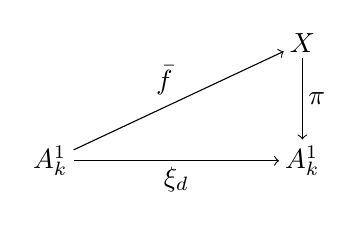
\begin{tikzpicture}[every node/.style={inner sep=2pt}]
  \node (A) at (0,0) {$\mathbb{A}^1_k$};
  \node (B) at (3.2,0) {$\mathbb{A}^1_k$};
  \node (C) at (3.2,1.5) {$X$};
  \draw[->] (A) -- node[above left] {$\bar f$} (C);
  \draw[->] (C) -- node[right] {$\pi$} (B);
  \draw[->] (A) -- node[below] {$\xi_d$} (B);
\end{tikzpicture}
\end{center}
且 $\bar f(0)=0$。若 $d=1$，这实际上不可能，因为 $\pi$ 的截面永远不会与纤维的奇点相交。另一方面，对 $d>1$，这是可能的，并且总存在唯一的环面爆破 $\tilde X\to X$，使得 $\bar f$ 提升为 $\tilde f:\mathbb{A}^1_k\to\tilde X$，且 $\tilde f(0)$ 位于例外除子的大环面轨道中。把所有这些映射限制到 $D^{\dagger}$ 与 $\operatorname{Spec} k^{\dagger}$ 上，就得到如上所述的映射 $f:\operatorname{Spec} k^{\dagger}\to D^{\dagger}$；而对数态射 $f$ 记住的正是需要哪一次环面爆破以及 $\tilde f(0)$ 是什么。\hfill$\square$
\end{example}

对数概形范畴一般过于宽泛：其中有许多非常病态的例子。一个关键概念是细对数结构。

% [原文 p.106]
\begin{definition}
设 $P$ 是幺半群，$X$ 是概形。用 $\underline{P}$ 表示 $X$ 上以 $P$ 为茎的常层，并设有一个前对数结构 $\underline{P}\to\mathcal{O}_X$。则称 $\underline{P}\to\mathcal{O}_X$ 为相应对数结构的\textbf{图表}（chart）。若存在映射 $\varphi:\underline{P}\to\mathcal{O}_X^{\times}$ 使得
\[
  \alpha_2(p)=\alpha_1(p)\cdot\varphi(p)\qquad \forall p\in P,
\]
则称两个图表 $\alpha_1:\underline{P}\to\mathcal{O}_X$、$\alpha_2:\underline{P}\to\mathcal{O}_X$ 是\textbf{等价}的。容易看出，等价的图表诱导同构的对数结构。

若存在一个 étale 开覆盖 $\{U_i\}$，使得在每个 $U_i$ 上存在有限生成整幺半群 $P_i$ 以及前对数结构 $\underline{P_i}\to\mathcal{O}_{U_i}$，其相伴的对数结构与从 $X$ 拉回的对数结构同构，则称 $X$ 上的对数结构是\textbf{细的}（fine）。

若幺半群 $P$ 是整的，且只要 $p\in P^{\mathrm{gp}}$ 与某个正整数 $m$ 满足 $mp\in P$ 就有 $p\in P$，则称 $P$ 是\textbf{饱和的}。

若 $X$ 上的对数结构是细的，且对所有 $\bar x\in X$，$\overline{\mathcal{M}}_{X,\bar x}$ 都是饱和的，则称该对数结构是\textbf{细饱和的}。
\end{definition}

% [Tutor Note: 定义 3.18 中的 $\underline{P}$ 是取值为 $P$ 的常层，不要与概形 $X$ 上作为 $\mathcal{O}_X$-模的 $\underline{P}$ 混淆；图表等价关系中的 $\varphi$ 取值于 $\mathcal{O}_X^{\times}$，因此等价的两个图表给出同构而非相同的对数结构。核对时可用例 3.19 的环面图表：把 $z^p$ 乘以单位 $\varphi(p)$ 不改变 $\alpha$ 的像所在的除子。]

\begin{example}
设 $P$ 是环面幺半群，即具有 $P=\sigma^{\vee}\cap N$ 的形式，其中 $\sigma\subseteq M_{\mathbb{R}}$ 是严格凸有理多面体锥；令 $X=X_{\sigma}=\operatorname{Spec} k[P]$。由
\[
  P\longrightarrow\Gamma(X,\mathcal{O}_X)=k[P],\qquad p\longmapsto z^p
\]
给出的映射诱导幺半群层的态射
\[
  \underline{P}\longrightarrow\mathcal{O}_X,
\]
从而在 $X$ 上诱导一个相伴的对数结构。

若 $\partial X$ 表示 $X$ 的\textbf{环面边界}，即 $X$ 中大环面轨道的补集，则事实上 $X$ 上的这个对数结构正是来自 $\partial X\subseteq X$ 的除子对数结构。确实，映射 $\underline{P}\to\mathcal{O}_X$ 通过
\[
  \underline{P}\longrightarrow\mathcal{M}_{(X,\partial X)}
  \xrightarrow{\ \alpha_X\ }\mathcal{O}_X
\]
分解，其中 $P\ni p\mapsto z^p\in\mathcal{M}_{(X,\partial X)}$，因为 $z^p$ 是 $X$ 上的正则函数，且在环面轨道 $X\setminus\partial X$ 上可逆。这给出映射
\[
  \underline{P}\oplus\mathcal{O}_X^{\times}\longrightarrow\mathcal{M}_{(X,\partial X)},
\]
其在开集 $U\subseteq X$ 上的核恰由满足 $z^{-p}$ 在 $U$ 上可逆的配对 $(p,z^{-p})$ 组成。此外，在 $x\in X$ 局部地，定义在 $x$ 的邻域 $U$ 上、且在 $U\setminus\partial X$ 上可逆的函数总具有 $\varphi\cdot z^p$ 的形式，其中 $\varphi$ 在 $U$ 上可逆、$p\in P$。因此 $\underline{P}\oplus\mathcal{O}_X^{\times}\to\mathcal{M}_{(X,\partial X)}$ 是满射，这说明此图表相伴的对数结构就是除子对数结构。\hfill$\square$
\end{example}

这个例子表明，$X$ 的（étale）开子集 $U$ 上的图表可以看成映射 $U\to\operatorname{Spec}\mathbb{Z}[P]$，使得 $U$ 上的对数结构是 $\operatorname{Spec}\mathbb{Z}[P]$ 上由环面边界诱导的除子对数结构的拉回。

\begin{example}
这里给出一个自然出现、但非细的对数结构的例子。令 $X=\operatorname{Spec} k[x,y,w,t]/(xy-wt)$，$D\subseteq X$ 为由 $t=0$ 给出的除子，诱导除子对数结构 $\mathcal{M}_{(X,D)}$。断言：该对数结构在 $0=(0,0,0,0)\in X$ 处不是细的。

% [原文 p.107]
事实上，假设存在 $0$ 的 étale 邻域 $U\to X$ 以及 $\mathcal{M}_{(X,D)}$ 的图表 $\underline{P}\to\mathcal{O}_U$。记 $\mathcal{M}_{(X,D)}$ 到 $U$ 的拉回为 $\mathcal{M}_U$，这意味着有同构 $(\underline{P}\oplus\mathcal{O}_U^{\times})/K\to\mathcal{M}_U$，其中模去 $K$ 定义前对数结构 $\underline{P}\to\mathcal{O}_U$ 相伴的对数结构。特别地，存在满射 $\underline{P}\to\overline{\mathcal{M}}_U$。它在茎上满，且对任意几何点 $\bar x\in U$ 有交换图表
\[
\begin{array}{ccc}
  P=\Gamma(U,\underline{P}) & \longrightarrow & \Gamma(U,\overline{\mathcal{M}}_U)\\[2pt]
  \big\downarrow\scriptstyle{\cong} & & \big\downarrow\scriptstyle{\cong}\\[2pt]
  P=\underline{P}_{\bar x} & \longrightarrow & \overline{\mathcal{M}}_{U,\bar x}
\end{array}
\]
因此 $\Gamma(U,\overline{\mathcal{M}}_U)\to\overline{\mathcal{M}}_{U,\bar 0}$ 必须是满射。

然而，若 $\varphi\in\mathcal{O}_{X,\bar 0}$ 是零点集包含于 $D$ 的函数，则 $\varphi=\psi\cdot t^n$，其中 $\psi\in\mathcal{O}_{X,\bar 0}^{\times}$。确实，在 $0$ 的邻域内，支撑在 $D$ 中的唯一 Cartier 除子是 $D$ 的倍数。于是存在非负整数 $n$，使得 $t^{-n}\cdot\varphi$ 不沿 $D$ 消失，从而由正规性，$t^{-n}\cdot\varphi$ 是可逆正则函数。因此 $\overline{\mathcal{M}}_{X,\bar 0}=\mathbb{N}\hookrightarrow\mathbb{N}^2$，即例 3.12 中的对角嵌入。另一方面，对 $X$ 中坐标满足 $x=y=0$ 且 $w\neq0$ 的点 $p$，$D$ 的两个不可约分支都是 Cartier 的，且 $\overline{\mathcal{M}}_{(X,D),\bar p}=\mathbb{N}^2$。于是存在 $0$ 的某个 étale 邻域，其上 $\Gamma(U,\overline{\mathcal{M}}_{(X,D)})=\mathbb{N}$，它不能满射到 $\overline{\mathcal{M}}_{(X,D),\bar p}=\mathbb{N}^2$。故该对数结构不可能是细的。\hfill$\square$
\end{example}

% [Tutor Note: 例 3.20 的非细性论证只用到一个局部事实：在 $0$ 的任意 étale 邻域 $U$ 上 $\Gamma(U,\overline{\mathcal{M}}_{(X,D)})=\mathbb{N}$，而在 $p=(0,0,w,0)$（$w\neq0$）处 $\overline{\mathcal{M}}_{(X,D),\bar p}=\mathbb{N}^2$；常层 $\underline{P}$ 在连通 $U$ 上的截面为 $P$，无法满射到 $\mathbb{N}^2$。注意 $X$ 是正规超曲面，故 $t^{-n}\varphi$ 的正则性由正规性（而非光滑性）保证。]

下一个概念常常有用：

\begin{definition}
态射 $f:X^{\dagger}\to Y^{\dagger}$ 是\textbf{严格的}（strict），若 $f^{\#}:f^{-1}\mathcal{M}_Y\to\mathcal{M}_X$ 诱导 $Y$ 上对数结构到 $X$ 的拉回与 $X$ 上对数结构之间的同构。
\end{definition}

\begin{examples}
\begin{enumerate}[label=(\arabic*),leftmargin=2.2em,itemsep=3pt]
\item 设 $f:X\to\mathbb{A}^1_k$ 是光滑态射，考虑 $X$ 与 $\mathbb{A}^1_k$ 上分别由 $f^{-1}(0)\subseteq X$ 与 $0\in\mathbb{A}^1_k$ 给出的除子对数结构。则 $f$ 是对数概形的严格态射。
\item 设 $X$ 由 $\mathbb{A}^1_k\times\mathbb{P}^1_k$ 在点 $(0,(1:0))$ 处的爆破得到，$f:X\to\mathbb{A}^1_k$ 为爆破的下映射（blow-down）再与到 $\mathbb{A}^1_k$ 的投影复合而成。给 $X$ 配备由
\[
  \bigl(\mathbb{A}^1_k\times\{(1:0)\}\bigr)\cup
  \bigl(\{0\}\times\mathbb{P}^1_k\bigr)\cup
  \bigl(\mathbb{A}^1_k\times\{(0:1)\}\bigr)
\]
的总变换给出的除子对数结构，并给 $\mathbb{A}^1_k$ 配备来自 $0\in\mathbb{A}^1_k$ 的除子对数结构。则作为对数概形的态射，$f$ 除在 $\mathbb{A}^1_k\times\{(1:0)\}$、$\mathbb{A}^1_k\times\{(0:1)\}$ 的真变换以及 $f^{-1}(0)$ 的二重点处之外，处处严格。\hfill$\square$
\end{enumerate}
\end{examples}

下面定义对数光滑性。与通常的概形态射一样，光滑性可以用无穷小提升准则来定义，在对数情形也可以给出同样的条件。不过，就实用而言，最好给出一个等价的定义。

\begin{definition}
细对数概形的态射 $f:X^{\dagger}\to Y^{\dagger}$ 称为\textbf{对数光滑}的，若在 $X$ 与 $Y$ 上 étale 局部地它可以嵌入交换图表
\[
\begin{array}{ccc}
  X & \longrightarrow & \operatorname{Spec}\mathbb{Z}[P]\\[2pt]
  \big\downarrow & & \big\downarrow\\[2pt]
  Y & \longrightarrow & \operatorname{Spec}\mathbb{Z}[Q]
\end{array}
\]
并满足以下性质：
\begin{enumerate}[label=(\arabic*),leftmargin=2.2em,itemsep=2pt]
\item 水平映射诱导 $X^{\dagger}$ 与 $Y^{\dagger}$ 的图表 $\underline{P}\to\mathcal{O}_X$ 与 $\underline{Q}\to\mathcal{O}_Y$。
\item 诱导态射 $X\to Y\times_{\operatorname{Spec}\mathbb{Z}[Q]}\operatorname{Spec}\mathbb{Z}[P]$ 是概形的光滑态射。
\item 右侧竖直箭头由幺半群同态 $Q\to P$ 诱导，且 $\ker(Q^{\mathrm{gp}}\to P^{\mathrm{gp}})$ 是有限群，$\operatorname{coker}(Q^{\mathrm{gp}}\to P^{\mathrm{gp}})$ 的挠部分也是有限群，二者的阶都在 $X$ 上可逆。这里 $P^{\mathrm{gp}}$ 表示 $P$ 的 Grothendieck 群，见 §3.1.1。
\end{enumerate}
\end{definition}

% [原文 p.108]
本书只关心特征零域上的概形，因此最后一条对我们不太重要。此外，多数时候 $P$ 与 $Q$ 都是环面幺半群，从而 $P^{\mathrm{gp}}$ 与 $Q^{\mathrm{gp}}$ 无挠。

% [Tutor Note: 定义 3.23 的 (3) 中两个群都要求“阶在 $X$ 上可逆”，在特征 $0$ 下自动成立，这正是正文说“最后一条不太重要”的原因。另：本页第 (3) 条末句“one checks easily that $f$ is log smooth”中的 $f$ 应为 $\pi$——本节只出现了 $\pi:\mathbb{P}_{\tilde\Delta}^{\dagger}\to(\mathbb{A}^1_k)^{\dagger}$ 这一记号，$f$ 无从指代。]

\begin{examples}
\begin{enumerate}[label=(\arabic*),leftmargin=2.2em,itemsep=3pt]
\item 取 $Y=\operatorname{Spec} k$ 带平凡对数结构，$Q=0$，$X=\operatorname{Spec} k[P]$，$P$ 为环面幺半群，于是 $X\cong Y\times_{\operatorname{Spec}\mathbb{Z}[Q]}\operatorname{Spec}\mathbb{Z}[P]$。给 $X$ 配备例 3.19 中由图表 $P\to k[P]$ 给出的对数结构。则 $X^{\dagger}$ 在 $\operatorname{Spec} k$ 上对数光滑。当然，环面簇 $X$ 在通常意义下不必在 $\operatorname{Spec} k$ 上光滑，所以这是对数结构“使” $X$ 光滑的第一个例子。
\item 设 $X=\operatorname{Spec} k[P]$，$Y=\operatorname{Spec} k[\mathbb{N}]$，并设给定 $\rho\in P$，$\rho\neq0$，通过 $1\mapsto\rho$ 定义映射 $\mathbb{N}\to P$。这诱导态射 $X\to Y$，它由 $\operatorname{Spec}\mathbb{Z}[P]\to\operatorname{Spec}\mathbb{Z}[\mathbb{N}]$ 基变换得到，因此在例 3.19 的对数结构下是对数光滑的。我们还可再做一次基变换
\[
\begin{array}{ccc}
  X_0 & \longrightarrow & X\\[2pt]
  \big\downarrow & & \big\downarrow\\[2pt]
  \operatorname{Spec} k & \longrightarrow & Y
\end{array}
\]
其中 $\operatorname{Spec} k$ 映到 $0\in Y=\mathbb{A}^1_k$。拉回 $X$ 与 $Y$ 上的对数结构，得到对数概形态射 $X_0^{\dagger}\to\operatorname{Spec} k^{\dagger}$，其中 $\operatorname{Spec} k^{\dagger}$ 是标准对数点。再次有
\[
  X_0\cong\operatorname{Spec} k\times_{\operatorname{Spec}\mathbb{Z}[\mathbb{N}]}\operatorname{Spec}\mathbb{Z}[P],
\]
故此映射对数光滑。

这正是对我们至关重要的例子：它说明奇异概形 $X_0^{\dagger}$ 上的对数结构如何使 $X_0^{\dagger}$ 实际上在 $\operatorname{Spec} k^{\dagger}$ 上光滑，尽管 $X_0$ 可能可约、甚至非既约！

\item 把 (2) 整体化，考虑例 3.6 的环面簇退化 $\pi:\mathbb{P}_{\tilde\Delta}\to\mathbb{A}^1_k$。于是我们得到由 $\partial\mathbb{P}_{\tilde\Delta}\subseteq\mathbb{P}_{\tilde\Delta}$ 与 $0\in\mathbb{A}^1_k$ 分别诱导的除子对数结构，给出对数态射
\[
  \pi:\mathbb{P}_{\tilde\Delta}^{\dagger}\longrightarrow(\mathbb{A}^1_k)^{\dagger}.
\]
映射 $\pi^{\#}:\pi^{-1}\mathcal{M}_{(\mathbb{A}^1_k,0)}\to\mathcal{M}_{(\mathbb{P}_{\tilde\Delta},\partial\mathbb{P}_{\tilde\Delta})}$ 只是函数的拉回。于是容易验证 $f$ 在 $\mathbb{P}_{\tilde\Delta}$ 的标准仿射开子集上对数光滑，且 $\pi$ 在这些仿射开子集上与上面的 (2) 一致。此外，把对数结构限制到 $\pi^{-1}(0)$ 与 $0$ 上，得到对数光滑态射
\[
  \pi^{-1}(0)^{\dagger}\longrightarrow\operatorname{Spec} k^{\dagger}.
\]
\end{enumerate}
\end{examples}

% [原文 p.109]
\begin{remark}
与通常概形的情形不同，对数光滑态射不必平坦。例如考虑由幺半群同态 $\mathbb{N}^2\to\mathbb{N}^2$，$(a,b)\mapsto(a+b,b)$ 定义的映射
\[
  X=\operatorname{Spec}\mathbb{Z}[\mathbb{N}^2]\longrightarrow Y=\operatorname{Spec}\mathbb{Z}[\mathbb{N}^2].
\]
这把 $X$ 描述为 $Y$ 在原点处爆破的一个开片，故不平坦。一般地，由整幺半群同态 $h:Q\to P$ 诱导的态射 $\operatorname{Spec}\mathbb{Z}[P]\to\operatorname{Spec}\mathbb{Z}[Q]$，若 $f$ 是整的，则是平坦的。整幺半群同态 $h$ 称为\textbf{整的}，若只要 $q_1,q_2\in Q$、$p_1,p_2\in P$ 且 $h(q_1)+p_1=h(q_2)+p_2$，就存在 $q_3,q_4\in Q$ 与 $p\in P$ 使得
\[
  p_1=h(q_3)+p,\qquad p_2=h(q_4)+p,\qquad q_1+q_3=q_2+q_4.
\]
称细对数概形的态射 $f:X^{\dagger}\to Y^{\dagger}$ 是\textbf{整的}，若诱导态射 $f^{\#}:\mathcal{M}_{Y,f(\bar x)}\to\mathcal{M}_{X,\bar x}$ 对所有 $\bar x\in X$ 都是整的。
\end{remark}

% [Tutor Note: 注 3.25 只断言“整 $\Rightarrow$ 平坦”，并未断言必要性，译文保留这一单向性；原文此句用 $f$ 指代该态射（前文未命名），按上下文应是 $h$ 的整性。三个等式合起来正是说 $h$ 的“纤维和”仍落在 $P$ 内，可与 §3.1 中整幺半群的定义对照；$(a,b)\mapsto(a+b,b)$ 的反例说明整性不可去掉。]

\begin{example}
在第 4 章中我们将需要用到对数光滑曲线。F. Kato 在 [64] 中给出了这类曲线的局部描述。精确描述如下。设 $f:C^{\dagger}\to W^{\dagger}$ 是对数光滑且整的、相对维数为 $1$ 的态射，$W=\operatorname{Spec}(A)$，其中 $(A,\mathfrak{m})$ 是代数闭域 $k$ 上的完备局部环。再设 $C^{\dagger}$ 与 $W^{\dagger}$ 是细饱和对数概形。设 $0\in W$ 是闭点，$Q=\overline{\mathcal{M}}_{W,\bar 0}$。必定存在图表 $\sigma:Q\to A$ 定义 $W$ 上的对数结构。设 $C_0$ 是 $f$ 在 $0\in W$ 上的纤维，$\bar x$ 是 $C_0$ 的几何点。则在 $\bar x$ 处 étale 局部地，$C^{\dagger}$ 同构于下列对数概形之一：
\begin{enumerate}[label=(\arabic*),leftmargin=2.2em,itemsep=3pt]
\item $V=\operatorname{Spec} A[u]$，其中对数结构由图表
\[
  Q\longrightarrow\mathcal{O}_V,\qquad q\longmapsto f^{*}\sigma(q)
\]
诱导。
\item $V=\operatorname{Spec} A[u,v]/(uv-t)$，其中 $t\in\mathfrak{m}$，对数结构由图表
\[
  \mathbb{N}^2\oplus_{\mathbb{N}}Q\longrightarrow\mathcal{O}_V,\qquad
  \bigl((a,b),q\bigr)\longmapsto u^a v^b f^{*}\sigma(q)
\]
诱导。这里纤维和用对角映射 $\mathbb{N}\to\mathbb{N}^2$ 以及由 $f$ 决定的同态 $\mathbb{N}\to Q$（$1\mapsto\alpha\in Q$，$\sigma(\alpha)=t$）定义。
\item $V=\operatorname{Spec} A[u]$，对数结构由图表
\[
  \mathbb{N}\oplus Q\longrightarrow\mathcal{O}_V,\qquad
  (a,q)\longmapsto u^a f^{*}\sigma(q)
\]
诱导。
\end{enumerate}

这三种情形应如下理解。在 (1) 型邻域中，态射实际上是光滑的而不只是对数光滑的，局部上没有由对数结构给出的有趣信息；对数结构只是底上对数结构的拉回。对 (2) 型邻域，$C_0$ 是结点。对 (3) 型邻域，$u=0$ 是截面 $W\to C$ 的像，可视为一个标记点；对数结构是底上拉回对数结构与除子 $u=0$ 相伴的除子对数结构之和。

我们把 $C$ 上 (1)、(2)、(3) 型的点分别称为\textbf{光滑点}、\textbf{二重点}与\textbf{对数标记点}。\hfill$\square$
\end{example}

\begin{example}
考虑上例中 $W=\operatorname{Spec} k$ 且带来自图表 $\mathbb{N}\to k$
\[
  n\longmapsto
  \begin{cases}
    1, & n=0,\\
    0, & n>0
  \end{cases}
\]
的标准对数结构时的二重点情形。

% [原文 p.110]
按例 3.26 的 (2)，$V=\operatorname{Spec} k[u,v]/(uv)$ 上对数结构的描述依赖于元素 $\alpha\in Q=\mathbb{N}$ 的选取。我们取其为整数 $e>0$（$e=0$ 的情形被 $\sigma(\alpha)=t$ 且 $t$ 在我们情形中为零这一要求排除）。

令
\[
  S_e:=\mathbb{N}^2\oplus_{\mathbb{N}}\mathbb{N},
\]
其中 $\mathbb{N}\to\mathbb{N}^2$ 是对角映射，$\mathbb{N}\to\mathbb{N}$ 是乘以 $e$ 的映射。这个幺半群将在下一章中证明特别重要。它可以用生成元
\[
  \alpha_1=\bigl((1,0),0\bigr),\qquad
  \alpha_2=\bigl((0,1),0\bigr),\qquad
  \rho=\bigl((0,0),1\bigr),\qquad
  \alpha_1+\alpha_2=e\rho
\]
来描述。它也是由 $\sigma^{\vee}\cap\mathbb{N}$ 给出的幺半群，其中 $\sigma\subseteq M_{\mathbb{R}}$ 是由 $(1,0)$ 与 $(1,e)$ 生成的锥；见例 3.1 的 (2)。另一种描述是：它是 $\mathbb{N}^2$ 中由 $\alpha_1=(e,0)$、$\alpha_2=(0,e)$ 与 $\rho=(1,1)$ 生成的子幺半群。

% [Tutor Note: $S_e=\mathbb{N}^2\oplus_{\mathbb{N}}\mathbb{N}$ 的三种描述互相印证：生成元关系 $\alpha_1+\alpha_2=e\rho$ 给出 $\mathbb{N}^3/(\alpha_1+\alpha_2-e\rho)$，而 $\sigma^{\vee}\cap N$ 与 $\mathbb{N}^2$ 的子幺半群 $\langle(e,0),(0,e),(1,1)\rangle$ 给出同构的幺半群。核对时可取 $e=1$：此时 $S_1\cong\mathbb{N}^2$，$V_e$ 光滑；$e=2$ 时 $V_e$ 是 $A_1$ 奇点的环面曲面。]

于是例 3.26 的 (2) 在本情形给出的图表为
\[
  S_e\longrightarrow k[u,v]/(uv),\qquad
  \bigl((a,b),c\bigr)\longmapsto
  \begin{cases}
    u^a v^b, & c=0,\\
    0, & c\neq0.
  \end{cases}
\]
注意由此图表诱导的对数结构可以这样理解：令 $V_e:=\operatorname{Spec} k[S_e]$。这是一个具有 $A_{e-1}$ 奇点的环面曲面，其环面边界由方程 $z^{\rho}=0$ 给出。于是上述图表诱导嵌入
\[
  V\hookrightarrow V_e,
\]
把 $V$ 与 $\partial V_e$ 等同起来。$V$ 上的对数结构便是由 $V\subseteq V_e$ 给出的除子对数结构限制到 $V$ 上。
\end{example}

\begin{example}
固定正整数 $e_1,e_2,w$，并设 $e_2=we_1$。设 $\zeta$ 是一个 $w$ 次单位根。考虑如下给出的两条曲线 $C_1,C_2$：
\[
  C_1=\operatorname{Spec} k[x,y]/(xy),\qquad
  C_2=\operatorname{Spec} k[u,v]/(uv),
\]
$C_1$ 与 $C_2$ 上的对数结构由如下图表给出：
\[
  S_{e_1}\longrightarrow k[x,y]/(xy),\qquad
  \bigl((a,b),c\bigr)\longmapsto
  \begin{cases}
    (\zeta x)^a y^b, & c=0,\\
    0, & c\neq0;
  \end{cases}
\]
\[
  S_{e_2}\longrightarrow k[u,v]/(uv),\qquad
  \bigl((a,b),c\bigr)\longmapsto
  \begin{cases}
    u^a v^b, & c=0,\\
    0, & c\neq0.
  \end{cases}
\]
注意 $\mathcal{M}_{C_i}$ 是 $S_{e_i}\oplus\mathcal{O}_{C_i}^{\times}$ 的商，因此给定 $\beta\in S_{e_i}$，$(\beta,1)$ 代表 $\mathcal{M}_{C_i}$ 的一个元素 $s_{\beta}$。于是 $\mathcal{M}_{C_i}$ 的任一截面都可写成 $\varphi\cdot s_{\beta}$，其中 $\varphi$ 可逆、$\beta\in S_{e_i}$。采用这一记号，设 $C_i^{\dagger}\to\operatorname{Spec} k^{\dagger}$ 由 $\mathcal{M}_{C_i}$ 中对应于 $\rho_i=\bigl((0,0),1\bigr)\in S_{e_i}$ 的截面 $s_{\rho_i}$ 给出。尽管 $C_1$ 的图表依赖于 $\zeta$ 的选取，但事实上对数概形 $C_1^{\dagger}$ 并不依赖此选取，因为任意两种 $\zeta$ 的选取给出等价的图表。然而，对数态射 $C_1^{\dagger}\to\operatorname{Spec} k^{\dagger}$ 确实依赖于此图表。

现在我们已经指定了对数曲线 $C_i^{\dagger}$（$i=1,2$）与对数光滑态射 $C_i^{\dagger}\to\operatorname{Spec} k^{\dagger}$。考虑由 $u\mapsto x^w$、$v\mapsto y^w$ 给出的概形态射 $f:C_1\to C_2$，
% [原文 p.111]
我们希望把它提升为对数概形的态射 $f^{\dagger}:C_1^{\dagger}\to C_2^{\dagger}$，给出交换图表
\begin{equation}
\begin{array}{ccc}
  C_1^{\dagger} & \xrightarrow{\ f^{\dagger}\ } & C_2^{\dagger}\\[4pt]
  \big\downarrow & & \big\downarrow\\[4pt]
  \operatorname{Spec} k^{\dagger} & \xrightarrow{\ =\ } & \operatorname{Spec} k^{\dagger}
\end{array}
\tag{3.4}
\end{equation}
为此需要确定使图表
\[
\begin{array}{ccc}
  f^{-1}\mathcal{M}_{C_2} & \xrightarrow{\ f^{\#}\ } & \mathcal{M}_{C_1}\\[4pt]
  \big\downarrow\scriptstyle{\alpha_{C_2}} & & \big\downarrow\scriptstyle{\alpha_{C_1}}\\[4pt]
  f^{-1}\mathcal{O}_{C_2} & \xrightarrow{\ f^{*}\ } & \mathcal{O}_{C_1}
\end{array}
\]
交换的映射 $f^{\#}$。

由于希望 (3.4) 交换，我们需要 $f^{\#}(s_{\rho_2})=s_{\rho_1}$。又注意
\[
  f^{*}\alpha_{C_2}\bigl(s_{((1,0),0)}\bigr)=f^{*}u=x^w,\qquad
  f^{*}\alpha_{C_2}\bigl(s_{((0,1),0)}\bigr)=f^{*}v=y^w.
\]
因此必须有
\[
  f^{\#}\bigl(s_{((1,0),0)}\bigr)=\varphi_x\cdot s_{((w,0),0)},\qquad
  f^{\#}\bigl(s_{((0,1),0)}\bigr)=\varphi_y\cdot s_{((0,w),0)},
\]
其中 $\varphi_x,\varphi_y$ 是 $C_1$ 上的可逆函数，且当 $x\neq0$ 时 $\varphi_x=1$，当 $y\neq0$ 时 $\varphi_y=1$。但由于
\begin{align*}
  s_{\rho_1}^{e_2}=f^{\#}\bigl(s_{\rho_2}^{e_2}\bigr)
  &=f^{\#}\bigl(s_{((1,0),0)}\cdot s_{((0,1),0)}\bigr)\\
  &=\varphi_x\varphi_y\,s_{((w,w),0)}\\
  &=\varphi_x\varphi_y\,s_{((0,0),we_1)}\\
  &=\varphi_x\varphi_y\,s_{\rho_1}^{e_2},
\end{align*}
必须有 $\varphi_x\cdot\varphi_y=1$，从而 $\varphi_x=\varphi_y=1$。

因此对数态射 $f^{\dagger}:C_1^{\dagger}\to C_2^{\dagger}$ 由数据 $C_1^{\dagger}\to\operatorname{Spec} k^{\dagger}$ 与 $C_2^{\dagger}\to\operatorname{Spec} k^{\dagger}$ 完全决定。

如何解释这些数据存在 $w$ 种不同选择？这些选择反映了我们可以用不同方式形变 $C_1$ 使其覆盖 $C_2$ 的标准形变。我们可以通过
\[
  X_2=\operatorname{Spec} k[u,v,t]/(uv-t^{e_2})\longrightarrow
  \mathbb{A}^1_k=\operatorname{Spec} k[t]
\]
来形变 $C_2$。若作代换 $u\mapsto x^w$、$v\mapsto y^w$，则可分解
\[
  x^w y^w-t^{e_2}=\prod_{i=1}^{w}\bigl(xy-\zeta^i t^{e_1}\bigr)
\]

% [原文 p.112]
其中 $\zeta$ 是一个本原 $w$ 次单位根。于是对每个 $1\le i\le w$ 有交换图表
\[
\begin{array}{ccc}
  X_1^i=\operatorname{Spec} k[x,y,t]/(xy-\zeta^i t^{e_1}) & \longrightarrow & X_2\\[4pt]
  \big\downarrow & & \big\downarrow\\[4pt]
  \mathbb{A}^1_k & \xrightarrow{\ =\ } & \mathbb{A}^1_k
\end{array}
\]
这里到 $\mathbb{A}^1_k=\operatorname{Spec} k[t]$ 的竖直映射由 $t\mapsto t$ 给出。这给出 $C_1$ 在给定 $C_2$ 形变之上的不同形变。我们把以下事实留作读者的练习：将此图表限制为 (3.4) 那样的图表后，由 $\zeta$ 的 $w$ 种选取得到 (3.4) 的 $w$ 种可能。这一点在第 4 章将很重要，因为这些不同的对数结构选取给出真正不同的稳定曲线。
\end{example}

% [Tutor Note: 例 3.28 的关键是区分“对数概形”与“对数态射”：$C_1^{\dagger}$ 只由图表的等价类决定，而 $C_1^{\dagger}\to\operatorname{Spec} k^{\dagger}$ 由具体图表（即 $\zeta$ 的选取）决定。这也解释了为什么第 4 章中同一族 $C_1$ 会给出 $w$ 条不同的稳定曲线；核对 (3.4) 时用 $s_{\rho_1}^{e_2}=s_{\rho_2}^{e_2}$ 追踪 $\zeta$ 的幂次最方便。]

\subsection{对数导子与微分}

我们终于回到引入对数结构的原始动机。我们将定义对数导子，在对数光滑情形导出对数切丛，并得到对数微分层。

设 $\pi:X^{\dagger}=(X,\mathcal{M}_X)\to S^{\dagger}=(S,\mathcal{M}_S)$ 是对数概形的态射。

\begin{definition}
$X^{\dagger}$ 在 $S^{\dagger}$ 上、取值于 $\mathcal{O}_X$-模层 $E$ 的\textbf{对数导子}是一个配对 $(\mathrm{D},\mathrm{Dlog})$，其中 $\mathrm{D}:\mathcal{O}_X\to E$ 是 $X$ 在 $S$ 上的通常导子，$\mathrm{Dlog}:\mathcal{M}_X^{\mathrm{gp}}\to E$ 是阿贝尔群层的同态，满足 $\mathrm{Dlog}\circ\pi^{\#}=0$；它们还满足相容性条件
\begin{equation}
  \mathrm{D}\bigl(\alpha_X(m)\bigr)=\alpha_X(m)\cdot\mathrm{Dlog}(m)
  \tag{3.5}
\end{equation}
对所有 $m\in\mathcal{M}_X$ 成立，其中 $\alpha_X:\mathcal{M}_X\to\mathcal{O}_X$ 是对数结构。

我们用 $\Theta_{X^{\dagger}/S^{\dagger}}$ 表示 $X^{\dagger}$ 在 $S^{\dagger}$ 上、取值于 $\mathcal{O}_X$ 的对数导子层。\hfill$\square$
\end{definition}

在许多情形下，对数导子 $(\mathrm{D},\mathrm{Dlog})$ 已由 $\mathrm{D}$ 决定。

\begin{proposition}
假设存在开的稠密子集 $U\subseteq X$ 使得 $\pi|_U:U^{\dagger}\to S^{\dagger}$ 是严格的，且 $E$ 没有支撑在 $X\setminus U$ 中的截面。则遗忘映射
\[
  (\mathrm{D},\mathrm{Dlog})\longmapsto\mathrm{D}
\]
从 $X^{\dagger}/S^{\dagger}$ 上取值于 $E$ 的对数导子层到 $X/S$ 上取值于 $E$ 的通常导子层是单射。
\end{proposition}

\begin{proof}[证明]
设 $V\subseteq X$ 是开子集。则每个 $m\in\mathcal{M}_X(U\cap V)$ 可写成 $h\cdot\pi^{\#}(n)$，其中 $h\in\mathcal{O}_X^{\times}$、$n\in\mathcal{M}_S$。因此 $\mathrm{Dlog}(m)$ 由 $\mathrm{D}$ 通过 (3.5) 决定。于是若 $\mathrm{D}=0$，则 $\mathrm{Dlog}|_U=0$；在关于 $E$ 的假设下这蕴含 $\mathrm{Dlog}=0$。
\end{proof}

% [Tutor Note: 式 (3.5) 中的 $\mathrm{Dlog}$ 取值于一般的 $\mathcal{O}_X$-模层 $E$，$\alpha_X(m)\cdot\mathrm{Dlog}(m)$ 是 $\mathcal{O}_X$ 通过 $\alpha_X(m)$ 作用在 $E$ 上；当 $E=\mathcal{O}_X$ 时它退化为通常的“对数导数” $m^{-1}dm$。命题 3.30 的证明只用 $m=h\cdot\pi^{\#}(n)$ 这一分解，故“$E$ 没有支撑在 $X\setminus U$ 的截面”这一假设不可省。]

于是我们常常可以把对数导子看作带有由对数结构决定的某种消失行为的通常导子：

\begin{example}
设 $X$ 是域 $k$ 上的正规整概形，$Y\subseteq X$ 是纯余维一子概形，给出 $X$ 上的除子对数结构 $\mathcal{M}_{(X,Y)}$。则 $\Theta_{X^{\dagger}/k}$ 由保持 $Y$ 的理想的通常导子组成。为看出这一点，首先注意若 $U\subseteq X\setminus Y$，则 $\mathcal{M}_X|_U=\mathcal{O}_X^{\times}$，故命题 3.30 的假设满足，$\Theta_{X^{\dagger}/k}$ 是 $\Theta_{X/k}$ 的子层。现在若 $(\mathrm{D},\mathrm{Dlog})$ 是对数导子且 $f\in\mathcal{I}_{Y/X}$，
% [原文 p.113]
则在 $Y$ 的某个不可约分支的一般点 $\eta$ 处，可写 $f=f'\cdot t^p$，其中 $t$ 是 $\mathcal{I}_{Y/X}$ 在 $\eta$ 处的生成元，$p>0$，$f'$ 是正则函数。则 $t$ 在 $\eta$ 的邻域内定义了 $\mathcal{M}_{(X,Y)}$ 的一个元素，故
\[
  \mathrm{D}f=t^p\mathrm{D}f'+pf't^{p-1}\mathrm{D}t
  =t^p\bigl(\mathrm{D}f'+pf'\mathrm{Dlog}\,t\bigr)
\]
在 $\eta$ 的邻域内属于 $\mathcal{I}_{Y/X}$。因此 $\mathrm{D}f$ 沿 $Y$ 的每个分支消失，从而属于 $\mathcal{I}_{Y/X}$。

反之，若 $\mathrm{D}$ 是保持 $\mathcal{I}_{Y/X}$ 的通常导子，则对 $f\in\mathcal{M}_{(X,Y)}$ 定义 $\mathrm{Dlog}\,f$ 为 $\mathrm{D}f/f$；再次像上面那样在 $Y$ 的一般点处立即验证它是正则函数。\hfill$\square$
\end{example}

\begin{examples}
\begin{enumerate}[label=(\arabic*),leftmargin=2.2em,itemsep=3pt]
\item 设 $P$ 是环面幺半群，$X=\operatorname{Spec} k[P]$，$X$ 上的对数结构由图表 $P\to k[P]$ 给出，等价地由除子对数结构 $\partial X\subseteq X$ 给出。有映射 $X^{\dagger}\to\operatorname{Spec} k$，其中 $\operatorname{Spec} k$ 带平凡对数结构。我们来计算 $\Theta_{X^{\dagger}/k}$。由例 3.31，它是通常导子层 $\Theta_{X/k}$ 中保持 $\partial X$ 的理想的子层。我们首先说明 $\partial X$ 的理想由单项式 $z^p$（$p\in\operatorname{Int}(P)$）生成。这里 $\operatorname{Int}(P)$ 的含义如下。由于 $P$ 是环面幺半群，它具有形式 $\sigma\cap P^{\mathrm{gp}}$，其中 $\sigma\subseteq P^{\mathrm{gp}}\otimes_{\mathbb{Z}}\mathbb{R}$ 是某个锥。则 $\operatorname{Int}(P)=\operatorname{Int}(\sigma)\cap P^{\mathrm{gp}}$。为看出为什么这是正确的理想，考虑对偶锥 $\sigma^{\vee}$。$X$ 的环面除子与 $\sigma^{\vee}$ 的一维面一一对应；对 $p\in P$，$z^p$ 在某个环面除子上消失当且仅当 $p$ 在 $\sigma^{\vee}$ 的对应边上非零。因此 $z^p$ 在所有环面除子上消失当且仅当 $p$ 在 $\sigma^{\vee}\setminus\{0\}$ 上处处非零，即 $p\in\operatorname{Int}(P)$。

现在考虑 $X$ 的大环面轨道 $X^o=\operatorname{Spec} k[M]$ 上的通常导子，其中 $M=P^{\mathrm{gp}}$，$N=\operatorname{Hom}_{\mathbb{Z}}(M,\mathbb{Z})$。$k[M]$ 的导子模可以等同于
\[
  \bigoplus_{m\in M} z^m\bigl(N\otimes_{\mathbb{Z}}k\bigr),
\]
其中 $z^m(n\otimes1)$ 是导子，记作 $z^m\partial_n$，其作用为
\[
  z^m\partial_n\bigl(z^{m'}\bigr)=\langle n,m'\rangle z^{m+m'}.
\]

现在这样的导子若保持 $k[P]$ 就延拓为 $k[P]$ 的导子；若它保持 $\partial X$ 的理想（由 $\{z^p\mid p\in\operatorname{Int}(P)\}$ 生成），就给出对数导子。于是我们来检验导子 $z^m\partial_n$。

显然，若 $m\in P$，则 $z^m\partial_n$ 既保持 $k[P]$ 又保持 $\partial X$ 的理想，因为 $P$ 与 $\operatorname{Int}(P)$ 对加上 $P$ 中元素封闭。

接下来，设 $m\notin P$。如上，设 $P$ 来自锥 $\sigma$。则 $\sigma^{\vee}$ 的某条边的本原生成元 $n$ 满足 $\langle n,m\rangle<0$。先设 $n'\in N$ 不与 $n$ 成比例，考虑 $z^m\partial_{n'}$。此时可找到 $m'\in P\cap n^{\perp}$ 使得 $\langle n',m'\rangle\neq0$，于是
\[
  z^m\partial_{n'}z^{m'}=\langle n',m'\rangle z^{m'+m}\neq0,
\]
且 $\langle n,m'+m\rangle<0$，故 $z^m\partial_{n'}$ 不保持 $k[P]$。

若 $n'$ 与 $n$ 成比例，可取 $n'=n$。存在 $m'\in\operatorname{Int}(P)$ 使得 $\langle n,m'\rangle=1$。但此时 $z^m\partial_n z^{m'}=z^{m+m'}$，且 $\langle n,m+m'\rangle\le0$。于是 $z^m\partial_n$ 不保持 $\partial X$ 的理想。

于是我们看到 $X$ 上对数导子的模为
\[
  \bigoplus_{p\in P} z^p\bigl(N\otimes_{\mathbb{Z}}k\bigr)=k[P]\otimes_{\mathbb{Z}}N.
\]
因此作为层，
\[
  \Theta_{X^{\dagger}/k}=\mathcal{O}_X\otimes_{\mathbb{Z}}N.
\]

% [原文 p.114]
\item 其次设有一个单项式 $z^{\rho}\in k[P]$ 诱导映射
\[
  X\longrightarrow\operatorname{Spec} k[\mathbb{N}]=\mathbb{A}^1_k,
\]
其中 $\mathbb{A}^1_k$ 上的对数结构由图表 $\mathbb{N}\to k[\mathbb{N}]$（等价地，由除子 $0\in\mathbb{A}^1_k$）诱导。我们得到对数光滑态射 $X^{\dagger}\to(\mathbb{A}^1_k)^{\dagger}$。则
\[
  \Theta_{X^{\dagger}/(\mathbb{A}^1_k)^{\dagger}}=\mathcal{O}_X\otimes_{\mathbb{Z}}\rho^{\perp}.
\]
确实，$\Theta_{X^{\dagger}/(\mathbb{A}^1_k)^{\dagger}}$ 恰是 $\Theta_{X^{\dagger}/k}$ 中零化 $\mathbb{A}^1_k$ 上函数的拉回（即零化 $z^{\rho}$）的导子构成的子模。\hfill$\square$
\end{enumerate}
\end{examples}

还存在泛对数导子，它引出对数微分层：

\begin{lemma}
给定对数概形的态射 $\pi:X^{\dagger}\to S^{\dagger}$，令
\[
  \Omega^1_{X^{\dagger}/S^{\dagger}}
  =\Bigl(\Omega^1_{X/S}\oplus\bigl(\mathcal{O}_X\otimes_{\mathbb{Z}}\mathcal{M}_X^{\mathrm{gp}}\bigr)\Bigr)\big/\mathcal{K},
\]
其中 $\mathcal{K}$ 是由
\[
  \bigl(d\alpha_X(m),-\alpha_X(m)\otimes m\bigr)
  \quad\text{与}\quad
  \bigl(0,1\otimes\pi^{*}(n)\bigr)
\]
（$m\in\mathcal{M}_X$，$n\in\mathcal{M}_S$）生成的 $\mathcal{O}_X$-模。则自然映射组成的配对 $(d,\mathrm{dlog})$
\[
  d:\mathcal{O}_X\xrightarrow{\ d\ }\Omega^1_{X/S}\longrightarrow\Omega^1_{X^{\dagger}/S^{\dagger}},
  \qquad
  \mathrm{dlog}:\mathcal{M}_X^{\mathrm{gp}}
  \xrightarrow{\ 1\otimes\cdot\ }
  \mathcal{O}_X\otimes\mathcal{M}_X^{\mathrm{gp}}
  \longrightarrow\Omega^1_{X^{\dagger}/S^{\dagger}}
\]
是泛对数导子。换言之，对任意 $\mathcal{O}_X$-模 $E$ 以及 $X^{\dagger}$ 在 $S^{\dagger}$ 上取值于 $E$ 的对数导子 $(\mathrm{D},\mathrm{Dlog})$，存在 $\mathcal{O}_X$-模映射 $\Phi:\Omega^1_{X^{\dagger}/S^{\dagger}}\to E$ 使得 $\mathrm{D}=\Phi\circ d$ 且 $\mathrm{Dlog}=\Phi\circ\mathrm{dlog}$。
\end{lemma}

\begin{proof}[证明]
先验证 $(d,\mathrm{dlog})$ 是对数导子。当然 $d$ 是通常导子。又
\[
  \bigl(d(\alpha_X(m)),-\alpha_X(m)\otimes m\bigr),\qquad
  \bigl(0,1\otimes(\pi^{\#}n)\bigr)\in\mathcal{K},
\]
从而 $d(\alpha_X(m))=\alpha_X(m)\mathrm{dlog}(m)$ 且 $\mathrm{dlog}\circ\pi^{\#}=0$，故 $(d,\mathrm{dlog})$ 是对数导子。

再验证泛性质。设 $(\mathrm{D},\mathrm{Dlog})$ 是取值于 $\mathcal{O}_X$-模层 $E$ 的对数导子：
\[
  \mathrm{D}:\mathcal{O}_X\longrightarrow E,\qquad
  \mathrm{Dlog}:\mathcal{M}_X^{\mathrm{gp}}\longrightarrow E.
\]
由 $\Omega^1_{X/S}$ 的泛性质，存在唯一态射 $\varphi:\Omega^1_{X/S}\to E$ 满足
\[
  \mathrm{D}=\varphi\circ d.
\]
定义
\[
  \Phi:\Omega^1_{X/S}\oplus\bigl(\mathcal{O}_X\otimes_{\mathbb{Z}}\mathcal{M}_X^{\mathrm{gp}}\bigr)
  \longrightarrow E,\qquad
  \Phi(\gamma,h\otimes m)=\varphi(\gamma)+h\cdot\mathrm{Dlog}(m).
\]
它下降为模去 $\mathcal{K}$ 的商，因为
\[
  \varphi\bigl(d\alpha_X(m)\bigr)-\alpha_X(m)\cdot\mathrm{Dlog}(m)=0,\qquad
  \mathrm{Dlog}\bigl(\pi^{\#}(n)\bigr)=0
\]
对每个 $m\in\mathcal{M}_X$、$n\in\mathcal{M}_S$ 成立。于是得到 $\Phi:\Omega^1_{X^{\dagger}/S^{\dagger}}\to E$。显然 $\Phi\circ d=\mathrm{D}$ 且 $\Phi\circ\mathrm{dlog}=\mathrm{Dlog}$。唯一性由 $\Omega^1_{X/S}\oplus(\mathcal{O}_X\otimes\mathcal{M}_X^{\mathrm{gp}})$ 作为 $\mathcal{O}_X$-模由 $\Omega^1_{X/S}$ 与 $1\otimes\mathcal{M}_X^{\mathrm{gp}}$ 生成得到；在这些子集上 $\Phi$ 分别由 $\varphi$ 与 $\mathrm{Dlog}$ 决定。
\end{proof}

$\mathcal{O}_X$-模 $\Omega^1_{X^{\dagger}/S^{\dagger}}$ 就是\textbf{对数微分层}。

% [原文 p.115]
\begin{remark}
首先注意，由泛性质有关系
\[
  \Theta_{X^{\dagger}/S^{\dagger}}
  =\mathcal{H}om_{\mathcal{O}_X}\bigl(\Omega^1_{X^{\dagger}/S^{\dagger}},\mathcal{O}_X\bigr).
\]
其次，若 $\alpha:\underline{P}\to\mathcal{O}_U$ 是 $X$ 上对数结构的图表，则在 $\Omega^1_{X^{\dagger}/S^{\dagger}}$ 的公式中可以把 $\mathcal{M}_X^{\mathrm{gp}}$ 换成 $P^{\mathrm{gp}}$、把 $\alpha_X$ 换成 $\alpha$。事实上，任意 $h\in\mathcal{O}_X^{\times}$ 给出关系
\[
  \bigl(dh,-h\otimes\alpha_X^{-1}(h)\bigr)\in\mathcal{K}.
\]
因此，对任意 $m\in P^{\mathrm{gp}}$，对数微分 $\bigl(0,1\otimes(\alpha_X^{-1}(h)\cdot m)\bigr)$ 可写成
\[
  h^{-1}(dh,0\otimes1)+(0,1\otimes m),
\]
即一个通常微分与一个只涉及 $m$ 的对数微分之和。\hfill$\square$
\end{remark}

\begin{definition}
给定 $S^{\dagger}$ 上对数概形的态射 $f:X^{\dagger}\to Y^{\dagger}$，存在自然的函子态射
\[
  f^{*}:f^{*}\Omega^1_{Y^{\dagger}/S^{\dagger}}\longrightarrow\Omega^1_{X^{\dagger}/S^{\dagger}},
\]
它由 $f^{*}:f^{*}\Omega^1_{Y/S}\to\Omega^1_{X/S}$ 与 $f^{*}\otimes f^{\#}:f^{-1}(\mathcal{O}_Y\otimes\mathcal{M}_Y^{\mathrm{gp}})\to\mathcal{O}_X\otimes\mathcal{M}_X^{\mathrm{gp}}$ 诱导。对偶地，这给出态射
\[
  f_{*}:\Theta_{X^{\dagger}/S^{\dagger}}\longrightarrow f^{*}\Theta_{Y^{\dagger}/S^{\dagger}}.
\]
\end{definition}

\begin{examples}
\begin{enumerate}[label=(\arabic*),leftmargin=2.2em,itemsep=3pt]
\item 如例 3.32，取 $X=\operatorname{Spec} k[P]$，$P$ 为环面幺半群，$X$ 带由标准图表 $P\to k[P]$ 给出的通常对数结构。考虑
\[
  \Omega^1_{X^{\dagger}/k}
  =\bigl(\Omega^1_{X/k}\oplus(\mathcal{O}_X\otimes_{\mathbb{Z}}P^{\mathrm{gp}})\bigr)\big/\mathcal{K}.
\]
注意 $\Omega^1_{X/k}$ 由形如 $d(z^p)$ 的微分生成，且
\[
  \bigl(d(z^p),-z^p\otimes p\bigr)\in\mathcal{K},
\]
故在 $\mathcal{K}$ 诱导的等价关系下，$\Omega^1_{X/k}$ 的每个元素都等价于 $\mathcal{O}_X\otimes P^{\mathrm{gp}}$ 中的元素。此外，$0\oplus(\mathcal{O}_X\otimes P^{\mathrm{gp}})$ 中没有 $\mathcal{K}$ 的非零元素，故 $\mathcal{O}_X\otimes P^{\mathrm{gp}}$ 单射入 $\Omega^1_{X^{\dagger}/k}$。因此
\[
  \Omega^1_{X^{\dagger}/k}=\mathcal{O}_X\otimes_{\mathbb{Z}}P^{\mathrm{gp}}
  =\mathcal{O}_X\otimes_{\mathbb{Z}}M,
\]
其中如前 $M=P^{\mathrm{gp}}$，$N=\operatorname{Hom}_{\mathbb{Z}}(M,\mathbb{Z})$。当然，这给出
\[
  \Theta^1_{X^{\dagger}/k}
  =\mathcal{H}om_{\mathcal{O}_X}\bigl(\Omega^1_{X^{\dagger}/k},\mathcal{O}_X\bigr)
  =\mathcal{O}_X\otimes_{\mathbb{Z}}N
\]
的一个更简单得多的计算。注意在此等同下，$\partial_n$ 是 $\Omega^1_{X^{\dagger}/k}$ 的对偶中在 $\mathrm{dlog}\,m$ 上取值 $\langle m,n\rangle$ 的元素。由于 $d(z^m)=z^m\mathrm{dlog}\,m$，我们看到 $\partial_n(d(z^m))=\langle m,n\rangle z^m$。这与例 3.32 (1) 中给出的 $\partial_n$ 的描述一致。

% [Tutor Note: 上式 $\Theta^{1}_{X^{\dagger}/k}$ 中的上标 $1$ 是原文笔误：由注 3.34 的第一式，切层应记作 $\Theta_{X^{\dagger}/k}$（不带 $1$），只有 $\Omega$ 带 $1$。这里照原文排版；引用时请以 $\Theta_{X^{\dagger}/k}$ 为准。]

\item 类似地，给定 $\rho\in P$，得到正则函数 $z^{\rho}:X\to\mathbb{A}^1_k$，它给出对数态射 $X^{\dagger}\to(\mathbb{A}^1_k)^{\dagger}$。把 $\mathcal{O}_X\otimes\mathbb{N}^{\mathrm{gp}}$ 在 $\mathcal{O}_X\otimes M$ 中的像除掉，就得到 $\Omega^1_{X^{\dagger}/(\mathbb{A}^1_k)^{\dagger}}$，即
\[
  \Omega^1_{X^{\dagger}/(\mathbb{A}^1_k)^{\dagger}}
  =\mathcal{O}_X\otimes_{\mathbb{Z}}M/\mathbb{Z}\rho.
\]
\item 我们可以进一步把 (2) 中的态射限制到零纤维上，得到对数态射 $X_0^{\dagger}\to\operatorname{Spec} k^{\dagger}$。此时注意，通过与 (1) 完全相同的论证有 $\Omega^1_{X_0^{\dagger}/k}=\mathcal{O}_{X_0}\otimes_{\mathbb{Z}}M$。于是
\[
  \Omega^1_{X_0^{\dagger}/k^{\dagger}}
  =\mathcal{O}_{X_0}\otimes_{\mathbb{Z}}M/\mathbb{Z}\rho,
\]
% [原文 p.116]
与 (2) 完全一样。

\item 若 $f:X^{\dagger}\to Y^{\dagger}$ 对数光滑，则 $\Omega^1_{X^{\dagger}/Y^{\dagger}}$ 局部自由：细节留给读者，可基于上面的例子。
\item 若 $X$ 是域 $k$ 上的非奇异簇，$D\subseteq X$ 是正规交叉除子，则得到 $X$ 上的除子对数结构 $\mathcal{M}_{(X,D)}$，且 $\Omega^1_{X^{\dagger}/k}\cong\Omega^1_X(\log D)$。这是 $j_{*}\Omega^1_{(X\setminus D)/k}$ 的子层（其中 $j:X\setminus D\hookrightarrow X$ 是包含），局部由
\[
  \frac{dx_1}{x_1},\ \dots,\ \frac{dx_p}{x_p},\ dx_{p+1},\ \dots,\ dx_n
\]
生成，其中 $x_1,\dots,x_n$ 是使 $D$ 由 $x_1\cdots x_p=0$ 给出的局部坐标。
\item 设 $C^{\dagger}\to\operatorname{Spec} k^{\dagger}$ 是对数光滑曲线，如例 3.26。则 $\Theta_{C^{\dagger}/k^{\dagger}}$ 是线丛。设 $C_0\subseteq C$ 是不可约分支。我们将通过描述 $\Theta_{C^{\dagger}/k^{\dagger}}|_{C_0}$ 来描述 $\Theta_{C^{\dagger}/k^{\dagger}}$。（若 $C$ 的亏格不为零，这不能完全确定 $\Theta_{C^{\dagger}/k^{\dagger}}$，因为在 $C$ 的二重点处粘合这些线丛有 $k^{\times}$ 的选择。）设 $x_1,\dots,x_n\in C_0$ 是 $C_0$ 中那些在 $C$ 中为二重点或为对数标记点的点。则断言
\[
  \Theta_{C^{\dagger}/k^{\dagger}}|_{C_0}
  \cong\Theta_{C_0/k}\Bigl(-\sum_{i=1}^{n}x_i\Bigr).
\]
确实，由命题 3.30，$\Theta_{C^{\dagger}/k^{\dagger}}$ 是 $\Theta_{C/k}$ 的子层。显然在 $C^{\dagger}\to\operatorname{Spec} k^{\dagger}$ 的光滑点处取得等号。

另一方面，我们来理解 $\Theta_{C^{\dagger}/k^{\dagger}}$ 在特殊点处的行为。在二重点 $x\in C$ 处，按例 3.28 的记号有 $\overline{\mathcal{M}}_{C,x}=S_e$（对某个 $e$）。于是 $C$ 及其对数结构可描述如下。令 $N=\mathbb{Z}^2$，$\sigma\subseteq N_{\mathbb{R}}$ 由 $(0,1)$ 与 $(e,1)$ 生成。则相应的环面簇 $X_{\sigma}$ 有正则函数 $z^{\rho}$，其中 $\rho=(0,1)\in M$，给出态射 $X_{\sigma}\to\mathbb{A}^1_k$。在 $x$ 附近，$C$ 是 $0\in\mathbb{A}^1_k$ 上的纤维，其对数结构由 $X_{\sigma}$ 上由 $\partial X_{\sigma}\subseteq X_{\sigma}$ 给出的除子对数结构诱导。因此我们恰处于上面例 3.36 (3) 的情形，局部地
\[
  \Theta_{C^{\dagger}/k^{\dagger}}
  =\operatorname{Hom}\bigl(\Omega^1_{C^{\dagger}/k^{\dagger}},\mathcal{O}_C\bigr)
  =\mathcal{O}_C\otimes_{\mathbb{Z}}\rho^{\perp}.
\]
当然，$\rho^{\perp}=\mathbb{Z}(1,0)\subseteq N$。

若 $n\in N$，我们把 $\Theta_{C^{\dagger}/k^{\dagger}}$ 中相应的对数导子记作 $\partial_n$，满足 $\partial_n(z^m)=\langle m,n\rangle z^m$。于是特别地，若在局部描述中写
\[
  C=\operatorname{Spec} k[z,w]/(zw)\subseteq\operatorname{Spec} k[z,w,t]/(zw-t^e),
\]
其中 $z=z^{(1,0)}$、$w=z^{(-1,e)}$、$t=z^{\rho}$，则 $\partial_{(1,0)}z=z$、$\partial_{(1,0)}w=-w$。于是若把此导子限制到 $C$ 的不可约分支 $C_0$ 上，比如可取 $C_0=V(w)$，就得到 $C_0=\operatorname{Spec} k[z]$ 上的导子 $z\partial_z$。因此 $\Theta_{C^{\dagger}/k^{\dagger}}$ 到 $C_0$ 的限制局部地由在原点处有一个零点的向量场层给出。

我们对对数标记点作类似分析。这里 $C$ 局部由指定 $\sigma\subseteq N_{\mathbb{R}}$（由 $(1,0)$ 与 $(0,1)$ 生成）并取 $\rho=(0,1)\in M$ 给出，于是 $\Theta_{C^{\dagger}/k^{\dagger}}$ 再次局部由 $\partial_{(1,0)}$ 生成。取 $z=z^{(1,0)}$、$t=z^{\rho}$，我们看到 $\partial_{(1,0)}=z\partial_z$ 作为通常导子成立，且 $C=C_0=\operatorname{Spec} k[z,t]/(t)$，故局部地 $\Theta_{C^{\dagger}/k^{\dagger}}|_{C_0}$ 再次由在对数标记点处有一个零点的向量场层组成。这就证明了断言。\hfill$\square$
\end{enumerate}
\end{examples}

% [Tutor Note: (6) 中 $\Theta_{C^{\dagger}/k^{\dagger}}|_{C_0}\cong\Theta_{C_0/k}(-\sum x_i)$ 只确定到二重点处的粘合；正文已指出亏格非零时有 $k^{\times}$ 的选择。二重点处的局部计算用 $\rho^{\perp}=\mathbb{Z}(1,0)$，故 $\partial_{(1,0)}$ 是唯一（至多相差一个非零数量倍）的对数导子；在 $C_0=V(w)$ 上它化为 $z\partial_z$，恰在原点为零，这就是 $(-x)$ 项的来源。]

% [原文 p.117]
\subsection{对数形变理论}

本节简要概述对数形变理论，细节与更一般的框架请参看 [65] 与 [63]。这里我们尽量使讨论相对简单，只做第 4 章所需的部分。

首先回顾光滑簇形变理论的基本想法。设给定 $\operatorname{Spec} k$ 上的光滑分离簇 $X$，我们想构造 $X$ 的 $k$ 阶形变。所谓 $k$ 阶形变，指的是如下数据。令 $R_k=k[t]/(t^{k+1})$，$\mathcal{O}_k=\operatorname{Spec} R_k$，故 $\mathcal{O}_0=\operatorname{Spec} k$。自然满射 $R_k\to R_{\ell}$（$\ell<k$）给出闭嵌入 $\mathcal{O}_{\ell}\to\mathcal{O}_k$。给定态射 $X_k\to\mathcal{O}_k$，$X_k$ 到 $\mathcal{O}_{\ell}$ 的限制是基变换 $X_k\times_{\mathcal{O}_k}\mathcal{O}_{\ell}\to\mathcal{O}_{\ell}$。于是 $X\to\operatorname{Spec} k$ 的 $k$ 阶形变就是一个平坦态射 $X_k\to\mathcal{O}_k$，使得 $X_k$ 到 $\mathcal{O}_0$ 的限制同构于 $X\to\operatorname{Spec} k$。

于是，若要构造 $X$ 的形变，我们逐步进行。假设已构造了 $(k-1)$ 阶形变 $X_{k-1}\to\mathcal{O}_{k-1}$，并希望把它提升为在 $\mathcal{O}_{k-1}$ 上限制到 $X_{k-1}$ 的形变 $X_k\to\mathcal{O}_k$。这可如下进行。

首先取 $X$ 的仿射开覆盖 $\{U_i\}$。令 $U_{ij}=U_i\cap U_j$。现在需要的第一个事实是：任意非奇异仿射簇 $U$ 的 $(k-1)$ 阶形变都是平凡的，即同构于 $U\times_k\mathcal{O}_{k-1}$。但给定 $X$ 的 $(k-1)$ 阶形变 $X_{k-1}$，$\mathcal{O}_{X_{k-1}}$ 到 $U_i$ 的限制诱导 $U_i$ 的 $(k-1)$ 阶形变 $U_i^{k-1}$。它必定平凡，即存在同构 $\theta_i^{k-1}:U_i^{k-1}\to U_i\times_k\mathcal{O}_{k-1}$。这给出粘合映射
\[
  \theta_{ij}^{k-1}:U_{ij}\times_k\mathcal{O}_{k-1}
  \longrightarrow U_{ij}\times_k\mathcal{O}_{k-1},
\]
它们由复合
\[
  U_{ij}\times_k\mathcal{O}_{k-1}
  \xrightarrow{\ (\theta_i^{k-1})^{-1}\ }
  U_{ij}^{k-1}
  \xrightarrow{\ \theta_j^{k-1}\ }
  U_{ij}\times_k\mathcal{O}_{k-1}
\]
定义。注意在 $U_{ij\ell}=U_i\cap U_j\cap U_{\ell}$ 上
\[
  \theta_{j\ell}^{k-1}\circ\theta_{ij}^{k-1}=\theta_{i\ell}^{k-1}.
\]

为构造 $X_k$，我们只需尝试提升这些等同，即选取等同
\[
  \theta_{ij}^{k}:U_{ij}\times_k\mathcal{O}_k\longrightarrow U_{ij}\times\mathcal{O}_k,
\]
使其限制到给定的 $\theta_{ij}^{k-1}$。这样的提升有很多，而提升的选取构成 $\Gamma(U_{ij},\Theta_{X/k})$ 上的一个挠子，其中 $\Theta_{X/k}$ 是 $X$ 的切丛，或取值于 $\mathcal{O}_X$ 的导子模。为明确看出这一点，考虑局部情形 $X=\operatorname{Spec} A$，并给定 $R_{k-1}$-代数同态 $f^{k-1}:A[t]/(t^k)\to A[t]/(t^k)$，它在模 $t$ 下是恒等。设 $f^k,\bar f^k$ 是 $f^{k-1}$ 到 $R_k$-代数同态 $A[t]/(t^{k+1})\to A[t]/(t^{k+1})$ 的两个提升。则对 $a\in A$ 有
\[
  \bar f^k(a)-f^k(a)=t^k\psi(a),
\]
其中 $\psi(a)\in A$。不难看出 $\psi$ 必定是 $A$ 的导子（参见命题 3.39 的证明）。此外，给定 $f^k$ 与导子 $\psi$，上式定义了 $\bar f^k$，而它是 $R_k$-代数同态这一事实来自 $\psi$ 是 $A$ 在 $k$ 上的导子。还注意，若 $f^{k-1}$ 是恒等，则存在 $f^{k-1}$ 的典范提升 $f^k$，即恒等；因此

% [原文 p.117 末句跨页；p.118 续："the set of all possible liftings … is identified canonically with Γ(X, Θ_{X/k})"，由下一块续译。]
% [Tutor Note: 本页 $\theta_{ij}^{k}:U_{ij}\times_k\mathcal{O}_k\to U_{ij}\times\mathcal{O}_k$ 中第二个纤维积漏了下标 $k$（原文如此），照排并注；否则它不是 $\mathcal{O}_k$-概形的态射，后文的挠子论证也无从谈起。]
